% Keep the appendix heading compact so both original screenshots fit below it.
% Restore the normal chapter-heading style immediately afterwards.
\makeatletter
\let\omnisound@normalchapterhead\@makechapterhead
\renewcommand{\@makechapterhead}[1]{%
  {\parindent\z@\raggedright\normalfont\LARGE\bfseries
   \@chapapp\space\thechapter:\space#1\par\nobreak\vskip12\p@}}
\makeatother
\chapter{Additional Prototype Screens}
\label{app:prototype-screens}
\makeatletter
\let\@makechapterhead\omnisound@normalchapterhead
\makeatother

This appendix shows additional screenshots from the two Omnisound prototypes. Chapter 4 focuses on particular controls and design changes, while these images provide a wider view of the interfaces.

\section{Home Screens}

Figure~\ref{fig:appendix-home} shows the Home screens from V1 and V2. Both versions include navigation and audio categories, while V2 places more emphasis on Continue Listening.

\begin{figure}[!htbp]
  \centering
  {\small\textbf{(a) V1 Home}\par}
  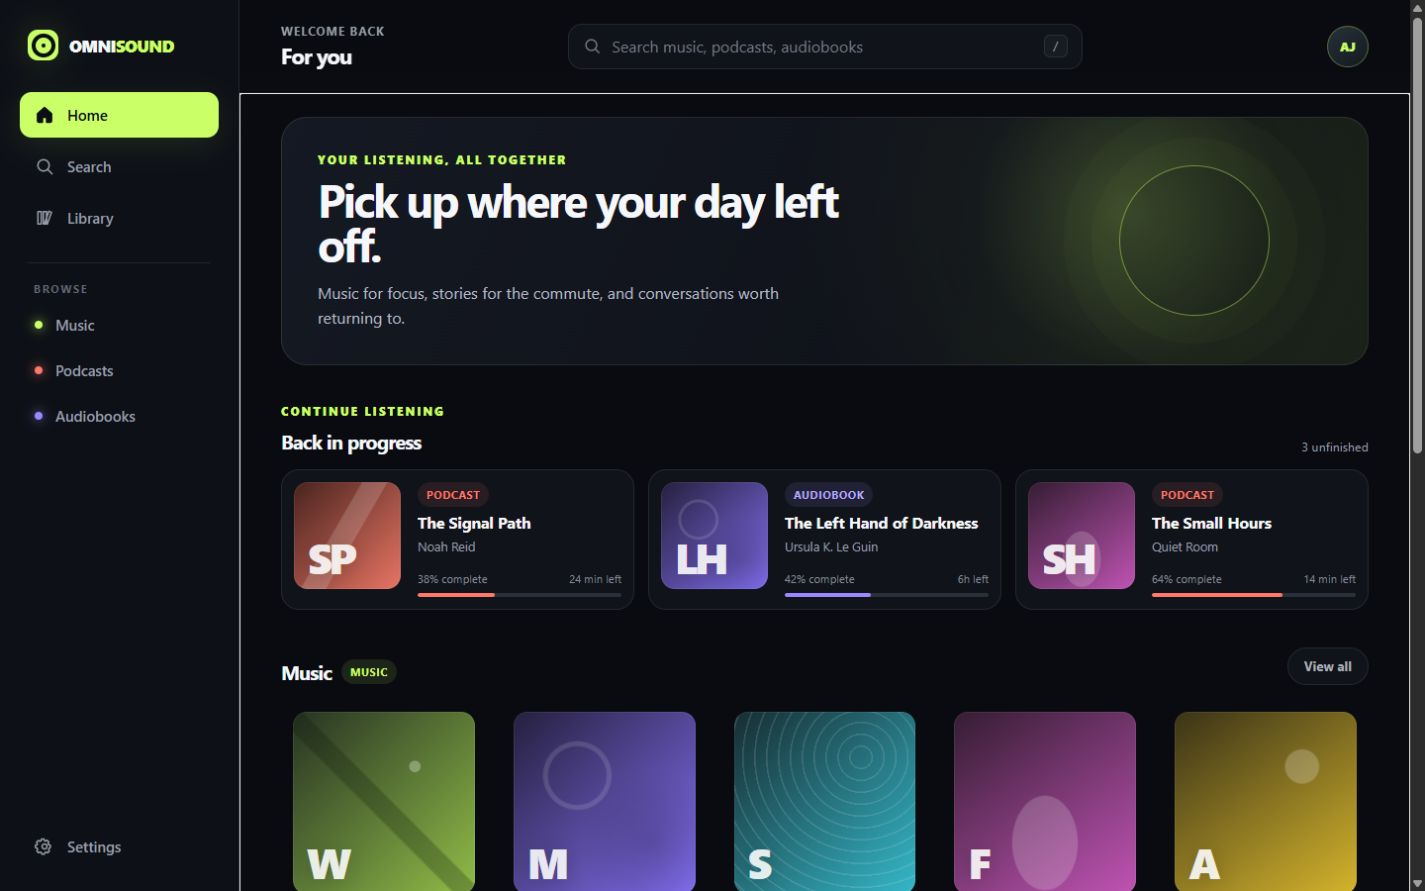
\includegraphics[width=\textwidth,height=0.30\textheight,keepaspectratio]{figures/v1/home.png}\par
  \vspace{3mm}
  {\small\textbf{(b) V2 Home}\par}
  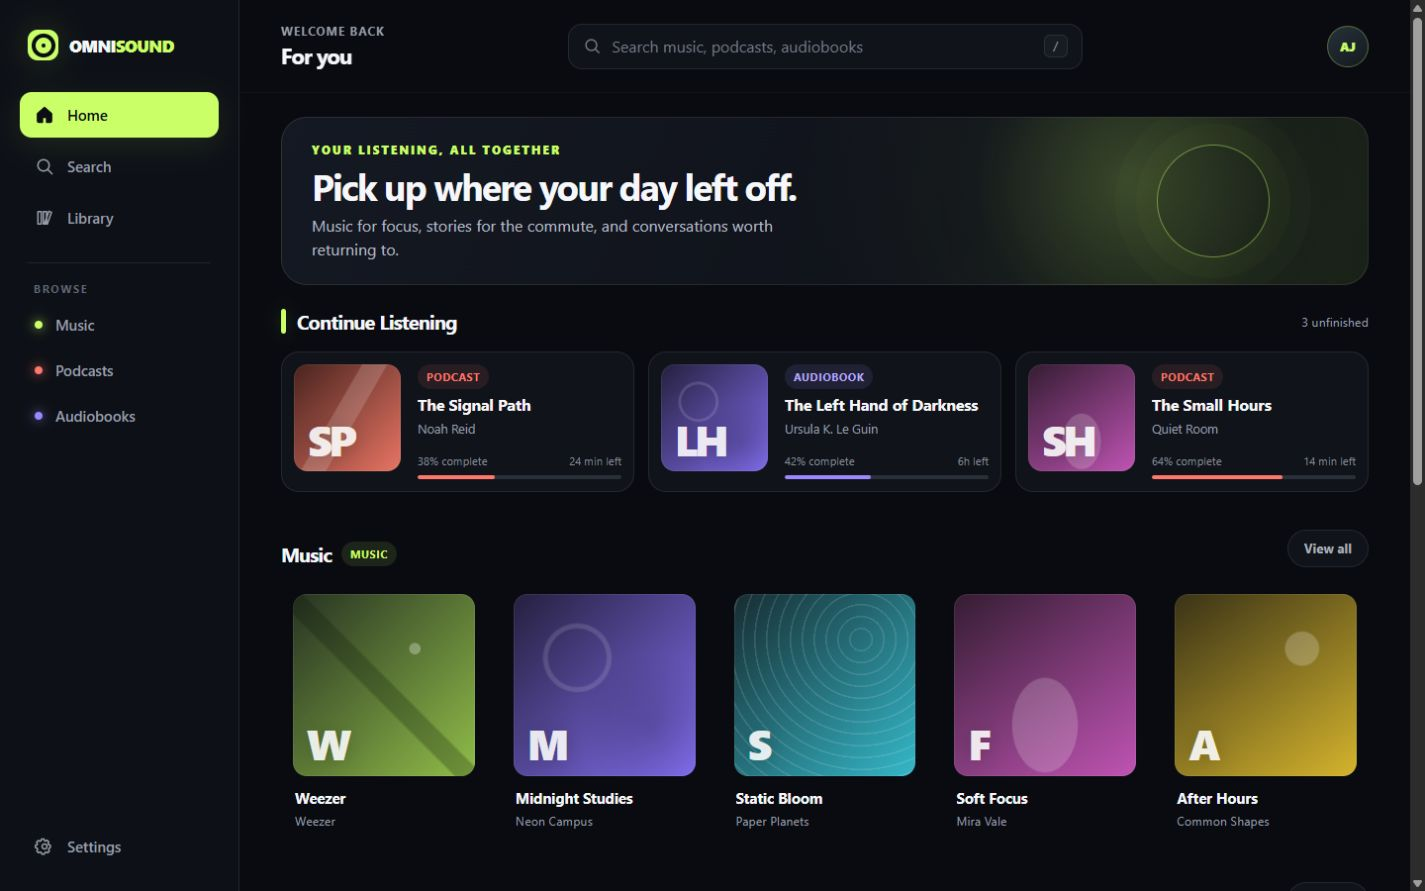
\includegraphics[width=\textwidth,height=0.30\textheight,keepaspectratio]{figures/v2/home.png}
  \caption{Home screens from the V1 and V2 prototypes.}
  \label{fig:appendix-home}
\end{figure}

\clearpage

\section{Library and Saving}

Figure~\ref{fig:appendix-library-saving} shows the V1 Library screen and a V2 content detail screen after an item has been saved. These are wider views of the interfaces discussed in the main report.

\begin{figure}[!htbp]
  \centering
  {\small\textbf{(a) V1 Library}\par}
  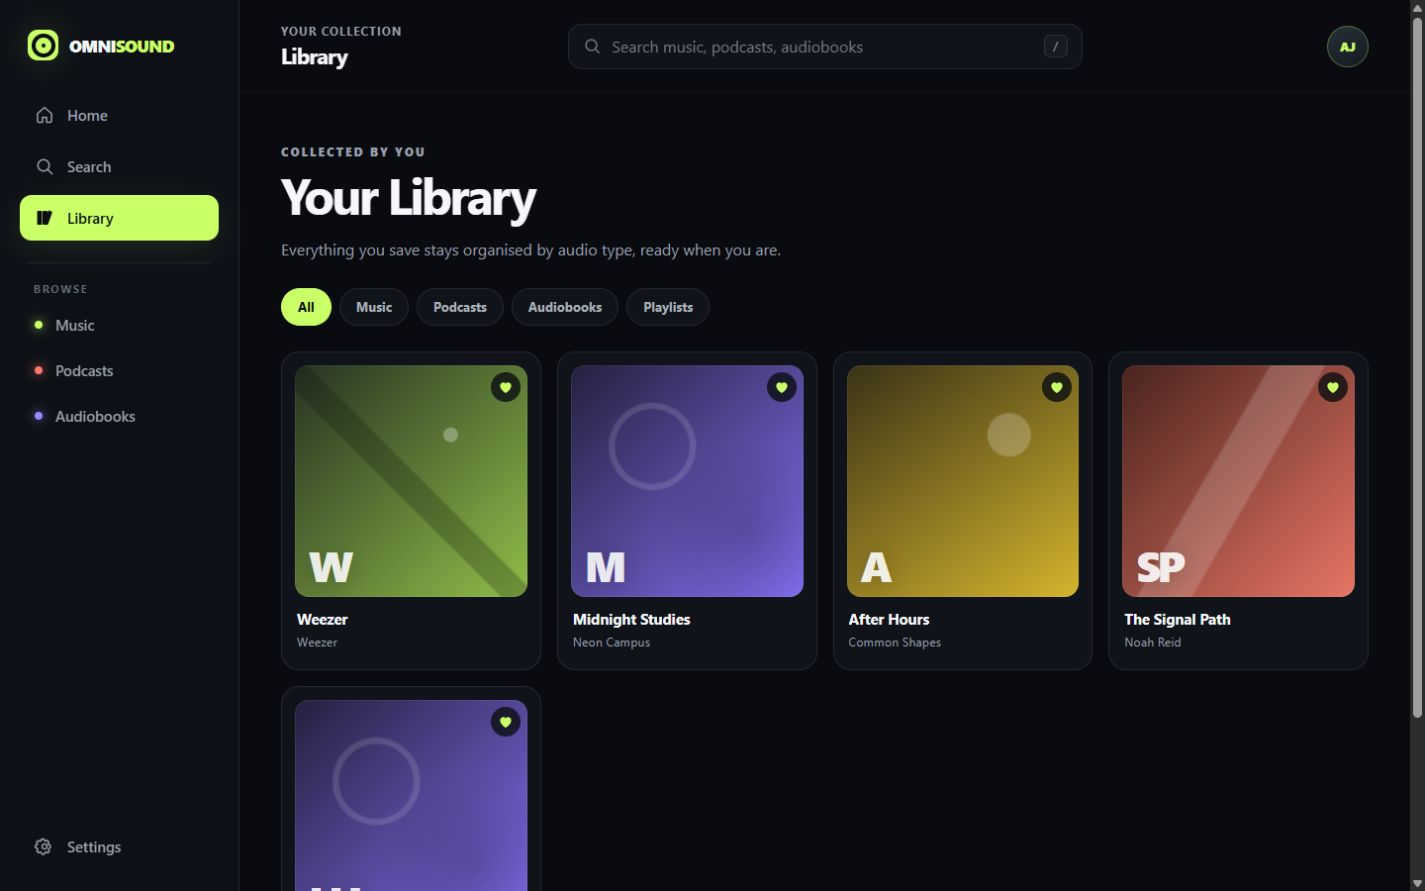
\includegraphics[width=\textwidth,height=0.32\textheight,keepaspectratio]{figures/v1/library.png}\par
  \vspace{3mm}
  {\small\textbf{(b) V2 Saved item detail}\par}
  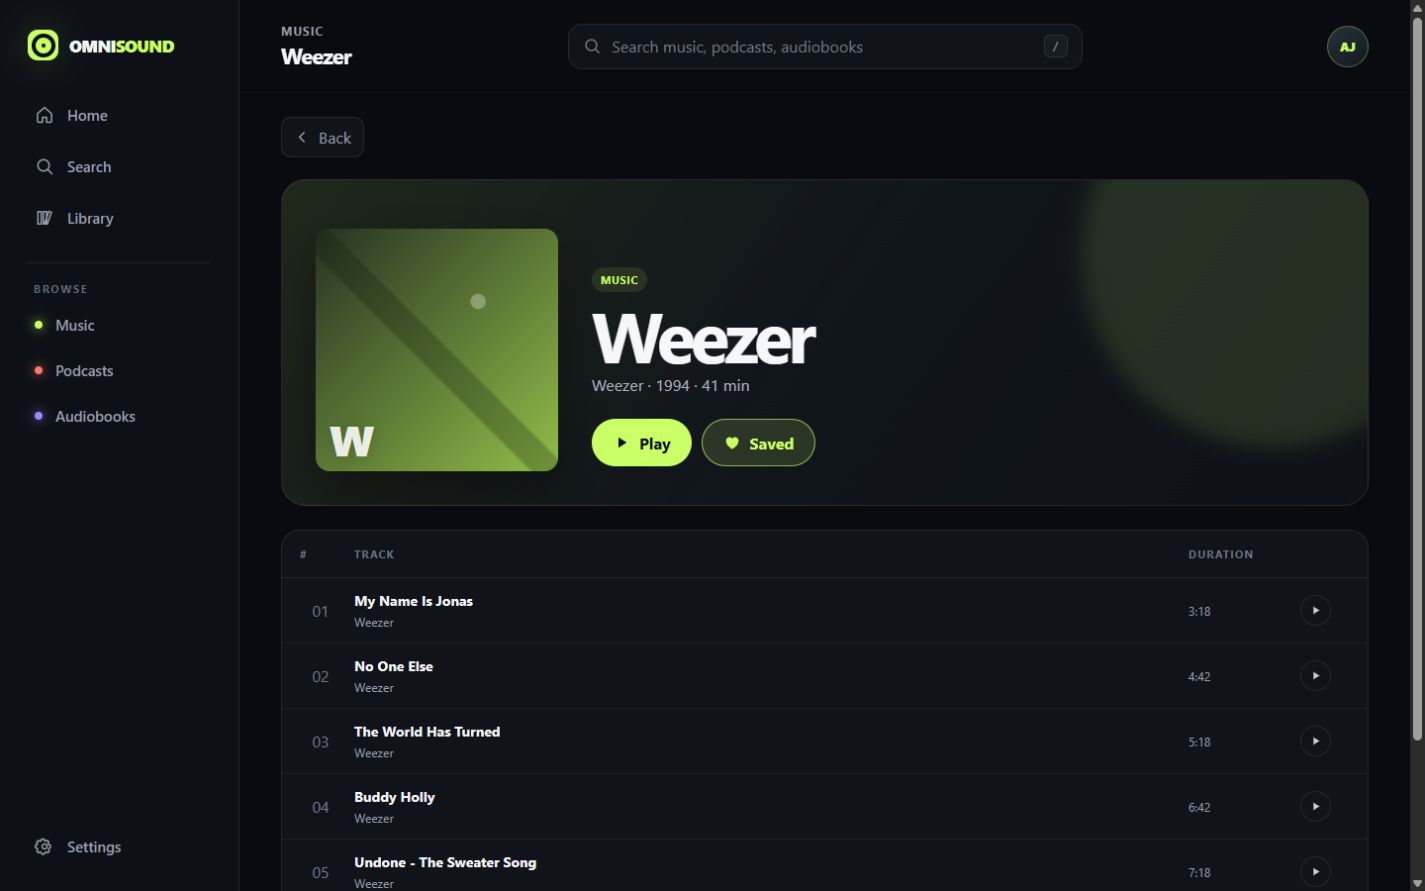
\includegraphics[width=\textwidth,height=0.32\textheight,keepaspectratio]{figures/v2/content-detail-saved.png}
  \caption{Additional interface views from V1 and V2.}
  \label{fig:appendix-library-saving}
\end{figure}
